\documentclass[tikz,border=8pt]{standalone}
\usepackage{tikz}
\usepackage{amsmath,amssymb}
\usetikzlibrary{arrows.meta,positioning,calc}

\begin{document}
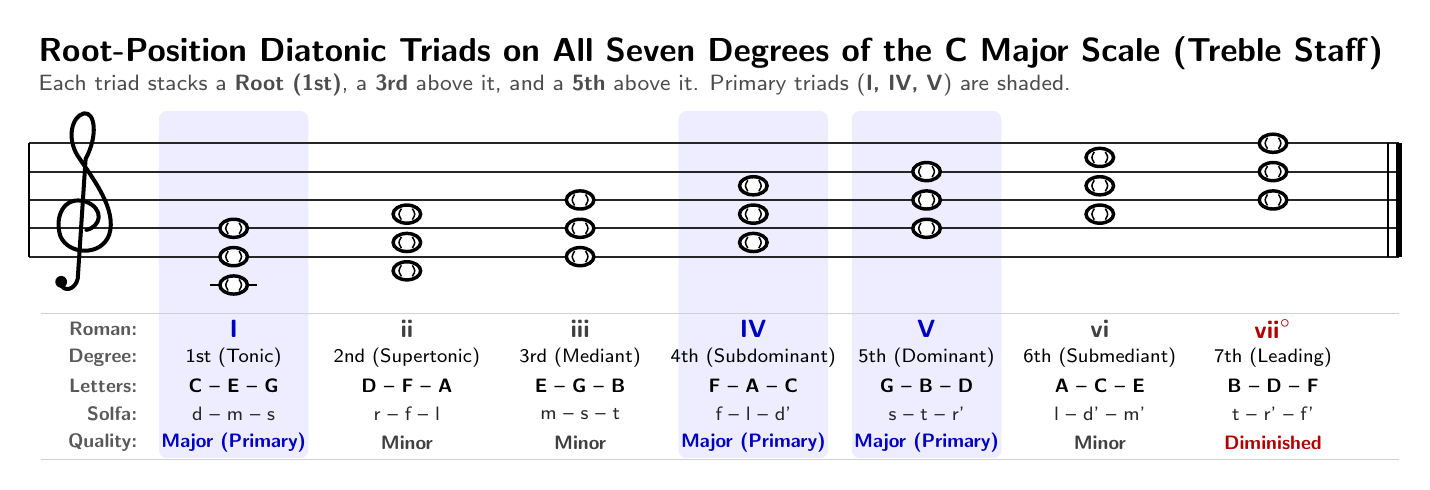
\begin{tikzpicture}[
    font=\sffamily,
    >=Stealth
]
% Staff lines at y = 0, 0.36, 0.72, 1.08, 1.44 (step d = 0.18 per scale step)
\def\staffL{0.0}
\def\staffR{17.4}

% Title banner
\node[font=\sffamily\bfseries\large, anchor=west] at (0, 2.58)
    {Root-Position Diatonic Triads on All Seven Degrees of the C Major Scale (Treble Staff)};
\node[font=\sffamily\footnotesize, text=black!70, anchor=west] at (0, 2.18)
    {Each triad stacks a \textbf{Root (1st)}, a \textbf{3rd} above it, and a \textbf{5th} above it. Primary triads (\textbf{I, IV, V}) are shaded.};

% Subtle highlight bands behind primary triads (I, IV, V)
\foreach \x in {2.6, 9.2, 11.4} {
    \fill[blue!7, rounded corners=3pt] (\x-0.95, -2.56) rectangle (\x+0.95, 1.85);
}

% Draw 5 staff lines
\foreach \k in {0,1,2,3,4} {
    \draw[line width=0.65pt, black!85] (\staffL, \k*0.36) -- (\staffR, \k*0.36);
}
\draw[line width=0.9pt] (\staffL, 0) -- (\staffL, 1.44);
\draw[line width=0.7pt] (\staffR-0.14, 0) -- (\staffR-0.14, 1.44);
\draw[line width=2.2pt] (\staffR, 0) -- (\staffR, 1.44);

% Treble Clef (G-clef) centred on line 2 (G4 = 0.36)
\begin{scope}[shift={(0.68, 0.36)}]
    \draw[line width=1.45pt, black, line cap=round, line join=round]
        (0.05, -0.02)
        .. controls (0.24, 0.02) and (0.28, 0.25) .. (0.04, 0.34)
        .. controls (-0.24, 0.42) and (-0.36, 0.14) .. (-0.28, -0.10)
        .. controls (-0.18, -0.34) and (0.24, -0.36) .. (0.34, -0.08)
        .. controls (0.44, 0.24) and (0.14, 0.62) .. (-0.06, 0.92)
        .. controls (-0.20, 1.14) and (-0.14, 1.42) .. (0.02, 1.46)
        .. controls (0.16, 1.48) and (0.20, 1.18) .. (0.04, 0.88)
        -- (-0.06, -0.64)
        .. controls (-0.09, -0.78) and (-0.24, -0.82) .. (-0.28, -0.70);
    \fill[black] (-0.27, -0.68) circle (0.075);
\end{scope}

% Semibreve (whole note) macro
\newcommand{\wholenote}[2]{%
    \fill[white] (#1, #2) ellipse (0.175 and 0.115);
    \draw[line width=1.25pt, black] (#1, #2) ellipse (0.175 and 0.115);
    \draw[line width=0.55pt, black] (#1-0.07, #2+0.07) .. controls (#1-0.11, #2) .. (#1-0.07, #2-0.07);
    \draw[line width=0.55pt, black] (#1+0.07, #2+0.07) .. controls (#1+0.11, #2) .. (#1+0.07, #2-0.07);
}

% Triad I: C4 - E4 - G4
\draw[line width=0.75pt] (2.6-0.30, -0.36) -- (2.6+0.30, -0.36);
\wholenote{2.6}{-0.36} \wholenote{2.6}{0.00} \wholenote{2.6}{0.36}
% Triad ii: D4 - F4 - A4
\wholenote{4.8}{-0.18} \wholenote{4.8}{0.18} \wholenote{4.8}{0.54}
% Triad iii: E4 - G4 - B4
\wholenote{7.0}{0.00} \wholenote{7.0}{0.36} \wholenote{7.0}{0.72}
% Triad IV: F4 - A4 - C5
\wholenote{9.2}{0.18} \wholenote{9.2}{0.54} \wholenote{9.2}{0.90}
% Triad V: G4 - B4 - D5
\wholenote{11.4}{0.36} \wholenote{11.4}{0.72} \wholenote{11.4}{1.08}
% Triad vi: A4 - C5 - E5
\wholenote{13.6}{0.54} \wholenote{13.6}{0.90} \wholenote{13.6}{1.26}
% Triad vii°: B4 - D5 - F5
\wholenote{15.8}{0.72} \wholenote{15.8}{1.08} \wholenote{15.8}{1.44}

% Row headings
\node[font=\sffamily\bfseries\scriptsize, anchor=east, text=black!65] at (1.50, -0.92) {Roman:};
\node[font=\sffamily\bfseries\scriptsize, anchor=east, text=black!65] at (1.50, -1.28) {Degree:};
\node[font=\sffamily\bfseries\scriptsize, anchor=east, text=black!65] at (1.50, -1.64) {Letters:};
\node[font=\sffamily\bfseries\scriptsize, anchor=east, text=black!65] at (1.50, -2.00) {Solfa:};
\node[font=\sffamily\bfseries\scriptsize, anchor=east, text=black!65] at (1.50, -2.36) {Quality:};

\foreach \x/\rom/\deg/\letn/\sol/\qual/\qcol in {
    2.6/{\textbf{I}}/{1st (Tonic)}/{C -- E -- G}/{d -- m -- s}/{Major (Primary)}/blue!75!black,
    4.8/{\textbf{ii}}/{2nd (Supertonic)}/{D -- F -- A}/{r -- f -- l}/{Minor}/black!75,
    7.0/{\textbf{iii}}/{3rd (Mediant)}/{E -- G -- B}/{m -- s -- t}/{Minor}/black!75,
    9.2/{\textbf{IV}}/{4th (Subdominant)}/{F -- A -- C}/{f -- l -- d'}/{Major (Primary)}/blue!75!black,
    11.4/{\textbf{V}}/{5th (Dominant)}/{G -- B -- D}/{s -- t -- r'}/{Major (Primary)}/blue!75!black,
    13.6/{\textbf{vi}}/{6th (Submediant)}/{A -- C -- E}/{l -- d' -- m'}/{Minor}/black!75,
    15.8/{\textbf{vii$^\circ$}}/{7th (Leading)}/{B -- D -- F}/{t -- r' -- f'}/{Diminished}/red!70!black%
} {
    \node[font=\sffamily\small, text=\qcol] at (\x, -0.92) {\rom};
    \node[font=\sffamily\scriptsize] at (\x, -1.28) {\deg};
    \node[font=\sffamily\bfseries\scriptsize] at (\x, -1.64) {\letn};
    \node[font=\sffamily\scriptsize, text=black!85] at (\x, -2.00) {\sol};
    \node[font=\sffamily\bfseries\scriptsize, text=\qcol] at (\x, -2.36) {\qual};
}

\draw[black!18, line width=0.4pt] (0.15, -0.72) -- (\staffR, -0.72);
\draw[black!18, line width=0.4pt] (0.15, -2.58) -- (\staffR, -2.58);

\end{tikzpicture}
\end{document}
